%%%%%%%%%%%%%%%%%%%%%%%%%%%%%%%%%%%%%%%%%%%%%%%%%%%%%%%%%%%%%%%%%%%%%%%%%%%
%% This file is part of the book
%%
%% Algorithmic Graph Theory
%% http://code.google.com/p/graph-theory-algorithms-book/
%%
%% Copyright (C) 2010 David Joyner <wdjoyner@gmail.com>
%% Copyright (C) 2009, 2010 Minh Van Nguyen <nguyenminh2@gmail.com>
%%
%% See the file COPYING for copying conditions.
%%%%%%%%%%%%%%%%%%%%%%%%%%%%%%%%%%%%%%%%%%%%%%%%%%%%%%%%%%%%%%%%%%%%%%%%%%%

\chapter{Distance and Connectivity}
\label{chap:distance_connectivity}


%%%%%%%%%%%%%%%%%%%%%%%%%%%%%%%%%%%%%%%%%%%%%%%%%%%%%%%%%%%%%%%%%%%%%%%%%%%

\section{Paths and distance}

\begin{itemize}
\item distance and metrics

\item distance matrix

\item eccentricity, center, radius, diameter

\item trees: distance, center, centroid

\item distance in self-complementary graphs
\end{itemize}


%%%%%%%%%%%%%%%%%%%%%%%%%%%%%%%%%%%%%%%%%%%%%%%%%%%%%%%%%%%%%%%%%%%%%%%%%%%

\subsection{Distance and metrics on graphs}

Consider an edge-weighted simple
graph $G=(V,E,i,h)$ without negative weight
cycles. Here $E\subset V^{(2)}$,
$i$ is an incidence function as in~\eqref{eqn:edge-incidence}, which
we regard as the identity function, and $h$ is an
orientation function as in~\eqref{eqn:edge-orientation}.
Let ${\rm wt}: E \to \R$ be the weight function.
(if $G$ is not provided with a weight function on the edges,
then assume that ${\rm wt}(e)=1$, for all $e\in E$.)
If $v_1,v_2\in V$ are two vertices and $P=(e_1,\dots,e_m)$ is
a path from $v_1$ to $v_2$ (so $v_1$ is incident to $e_1$
nd $v_2$ is incident to $e_m$), we define the {\it weight of $P$}
to be the sum of the weights of the edges in $P$:

\[
{\rm wt}(P)=\sum_{i=1}^m {\rm wt}(e_i).
\]
The {\it distance function} $\partial:V\times V \to  \R\cup
\{\infty\}$ on
\index{distance function}
$G$ is defined by $\partial(v_1,v_2) = \infty$,
if $v_1$ and $v_2$ lie in distinct connected
components of $G$, and by

\[
\partial(v_1,v_2) =
\min_P {\rm wt}(P),
\]
otherwise, where the minimum is taken over all paths $P$
from $v_1$ to $v_2$ (this minimum exists since
$G$ has no negative weight cycles.

This distance function is not in general a metric
(that is, the triangle inequality is not true in general).
However, when the distance function is a
metric then $G$ is called a {\it metric graph}.
\index{graph!metric}
The theory of metric graphs, thanks to their close
connection with tropical curves, is a very active
research area at the present (see the work of
M. Baker et al, e.g., \cite{BakerFaber2006}).

\begin{exercise}
Show that the vertex set $V$ (of an undirected unweighted simple graph)
and the distance function form
a metric space, if and only if the graph is connected.
\end{exercise}

The {\it eccentricity} $\epsilon:V \to  \R$ is defined as follows:
$\epsilon (v)$ (for a vertex $v$) is the greatest distance between $v$
and any other vertex in $G$.
\index{eccentricity}

The {\it diameter} of $G$, $\partial(G)$, is the maximum
eccentricity of any vertex in the graph. To compute
$\partial(G)$, first find the shortest path (see Chapter
\ref{chap:graph_algorithms}) between each pair of
vertices. The maximum weight of any of
these paths is the diameter of the graph:

\[
\partial(G) = \max_{v_1,v_2\in V} \partial(v_1,v_2).
\]
\index{diameter}

To compute the diameter of a graph, use the Floyd-Roy-Warshall
algorithm to compute the shortest distance between any
two pairs of vertices. The maximum of these distances is the
diameter.


%%%%%%%%%%%%%%%%%%%%%%%%%%%%%%%%%%%%%%%%%%%%%%%%%%%%%%%%%%%%%%%%%%%%%%%%%%%

\subsection{Distance matrix}

There are two uses of this term in the literature.

Consider an edge-weighted graph $G=(V,E)$ without negative weight
cycles with distance function $\partial$. Let $d=\partial(G)$
denote the diameter of $G$ and index the
set of vertices in some arbitrary but fixed way,
$V=\{v_1,v_2,\dots, v_n\}$.
The {\it distance matrices} of $G$ are a sequence of $n\times n$ matrices
$\{A_1,\dots, A_d)$, where

\[
(A_k)_{ij} =
\left\{
\begin{array}{ll}
1,& {\rm if}\ \partial(v_i,v_j)=k,\\
0,& {\rm otherwise}.
\end{array}
\right.
\]
In particular, $A_1$ is the usual adjacency matrix $A$.

To compute the distance matrices of a graph, use the Floyd-Roy-Warshall
algorithm to compute the shortest distance
$\partial(v_i,v_j)$ between any two pairs of vertices,
$v_i,v_j\in V$. This data determines the entries of
the distance matrices.

\begin{lstlisting}
def distance_matrices(Gamma):
    """
    Returns the distance matrices of a graph.

    INPUT:
        Gamma is a graph.
    OUTPUT:
        The sequence of distance matrices

    EXAMPLES:
        sage: A = matrix([[0,1,1,0,0],[1,0,1,0,0],[1,1,0,1,0],[0,0,1,0,1],[0,0,0,1,0]])
        sage: G = Graph(A, format = "adjacency_matrix", weighted = True)
        sage: print distance_matrices(G)
        [[1 0 0 0 0]
         [0 1 0 0 0]
         [0 0 1 0 0]
         [0 0 0 1 0]
         [0 0 0 0 1],
         [0 1 1 0 0]
         [1 0 1 0 0]
         [1 1 0 1 0]
         [0 0 1 0 1]
         [0 0 0 1 0],
         [0 0 0 1 0]
         [0 0 0 1 0]
         [0 0 0 0 1]
         [1 1 0 0 0]
         [0 0 1 0 0],
         [0 0 0 0 1]
         [0 0 0 0 1]
         [0 0 0 0 0]
         [0 0 0 0 0]
         [1 1 0 0 0]]
    """
    g = Gamma.diameter()
    V = Gamma.vertices()
    n = len(V)
    D = G.distance_all_pairs()
    dist_mats = []
    for i in range(g+1):
        dist_mati = [[0 for j in range(n)] for k in range(n)]
        for v1 in V:
            for v2 in V:
                if D[v1][v2]==i:
                    dist_mati[v1][v2] = 1
        dist_mats.append(matrix(dist_mati))
    return dist_mats
\end{lstlisting}

The {\it distance matrix} $D(G)$ of $G$ is
the $n\times n$ matrix

\[
D(G)=(\partial(v_j,v_j))_{1\leq i,j\leq n}.
\]
The distance matrix arises in several applications, including
communication network design (see for example
\cite{GrahamPollak1971})
and network flow algorithms (see for example \cite{Dijkstra1959}).

To compute the distance matrix of a graph, is very
similar to computing the distance matrices.
Again, use the Floyd-Roy-Warshall
algorithm to compute the shortest distance
$\partial(v_i,v_j)$ between any two pairs of vertices,
$v_i,v_j\in V$. This data determines the entries of
the distance matrix.

% R. L. Graham and H. O. Pollak, {\it on the addressing problem for
% loop switching}, Bell Tech J 50(1971)2495-2519.
% and
% E. W. Dijkstra, {\it A note on two problems in connection with
% graphs}, Numer. Math. 1 (1959)269-271.
% [(this is [Dijkstra1959] )!
\begin{remark}
{\rm
Thanks to R. Graham and H. Pollak, the following unusual fact is
known:
If $T$ is any tree then

\[
\det D(T)=(-1)^{n-1}(n-1)2^{n-2},
\]
where $n$ denotes the number of vertices of $T$.
In particular, the determinant of the distance matrix of a tree is
independent of the structure of the tree.  This fact is proven in the
paper \cite{GrahamPollak1971}, but see also
\cite{EdelbergEtAl1976}.
}
\end{remark}
% this lemma is proven in the above paper by Graham-Pollak
% see however:
% M. Edelberg, M. R. Garey, R. L. Graham, {\it On the
% distance matrix of a tree}, Discrete Math. 14 (1976)23-39.

\begin{lstlisting}
def distance_matrix(Gamma):
    """
    Returns the distance matrix of a graph.

    INPUT:
        Gamma is a graph.
    OUTPUT:
        The distance matrix

    EXAMPLES:
        sage: A = matrix([[0,1,1,0,0],[1,0,1,0,0],[1,1,0,1,0],[0,0,1,0,1],[0,0,0,1,0]])
        sage: G = Graph(A, format = "adjacency_matrix", weighted = True)
        sage: distance_matrix(G)
        [0 1 1 2 3]
        [1 0 1 2 3]
        [1 1 0 1 2]
        [2 2 1 0 1]
        [3 3 2 1 0]
    """
    g = Gamma.diameter()
    V = Gamma.vertices()
    n = len(V)
    D = G.distance_all_pairs()
    for i in range(g+1):
        dist_mat = [[0 for j in range(n)] for k in range(n)]
        for v1 in V:
            for v2 in V:
                dist_mat[v1][v2] = D[v1][v2]
    return matrix(dist_mat)
\end{lstlisting}


%%%%%%%%%%%%%%%%%%%%%%%%%%%%%%%%%%%%%%%%%%%%%%%%%%%%%%%%%%%%%%%%%%%%%%%%%%%

\section{Vertex and edge connectivity}

\begin{itemize}
\item vertex-cut and cut-vertex

\item cut-edge or bridge

\item vertex and edge connectivity
\end{itemize}

If $G=(V,E)$ is a graph and $v\in V$ is a vertex with the property
that $G-v$ has more connected components than $G$ then
we call $v$ a {\it cut-vertex} (or {\it articulation point} or {\it vertex-cut}).
\index{cut-vertex}
\index{vertex-cut}
\index{articulation point}
A {\it non-separable graph} is one having no cut-vertex.
\index{non-separable graph}
\index{graph!non-separable}
Otherwise, the graph is called {\it separable}.
\index{graph!separable}
A {\it block} of a graph is a maximal non-separable subgraph.
\index{block}

\begin{example}
{\rm
The cut-vertex of the graph in Figure~\ref{fig:distance_connectivity:claw_graph}
is the vertex $0$, as the following Sage example
demonstrates.

\begin{lstlisting}
sage: G = graphs.clawgraph()
sage: G.blocks_and_cut_vertices()
([[1, 0], [2, 0], [3, 0]], [0])
\end{lstlisting}

\begin{figure}[!htbp]
\centering
%%%%%%%%%%%%%%%%%%%%%%%%%%%%%%%%%%%%%%%%%%%%%%%%%%%%%%%%%%%%%%%%%%%%%%%%%%%
%% This file is part of the book
%%
%% Algorithmic Graph Theory
%% http://code.google.com/p/graph-theory-algorithms-book/
%%
%% Copyright (C) 2009, 2010, 2011 Minh Van Nguyen <nguyenminh2@gmail.com>
%%
%% See the file COPYING for copying conditions.
%%%%%%%%%%%%%%%%%%%%%%%%%%%%%%%%%%%%%%%%%%%%%%%%%%%%%%%%%%%%%%%%%%%%%%%%%%%

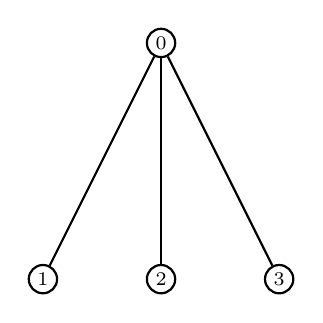
\begin{tikzpicture}
[nodeDecorate/.style={shape=circle,inner sep=1.5pt,draw,thick},%
  lineDecorate/.style={-,thick},%
  scale=1.5]
\scriptsize
%% nodes or vertices
\foreach \nodename/\x/\y in {1/0/0, 2/1/0, 3/2/0, 0/1/2}
{
  \node (\nodename) at (\x,\y) [nodeDecorate] {$\nodename$};
}
%% edges or lines
\path
\foreach \startnode/\endnode in {0/1, 0/2, 0/3} {
  (\startnode) edge[lineDecorate] node {} (\endnode)
};
\end{tikzpicture}

\caption{A claw graph with $4$ vertices.}
\label{fig:distance_connectivity:claw_graph}
\end{figure}
}
\end{example}

If $G$ has at least $3$ vertices and there is a $v\in V$
which is a cut-vertex then we say $G$ is {\it $1$-connected}.
\index{graph!$1$-connected}
 In general, we say $G$ is {\it $k$-vertex-connected} (or
{\it $k$-connected})
\index{vertex-connected}
if the graph $G-X$ is connected for each $X\subset V$
such that $|X|\leq k-1$.
In other words, $G$ is $k$-vertex-connected
if the graph remains connected even after removing
any $k-1$ or fewer vertices from $G$.

\begin{example}
The $1$-skeleton of any $k$-dimensional convex polytope forms
a $k$-vertex-connected graph
(\cite{Balinski1961}). As a partial converse, Steinitz's theorem
states that any $3$-vertex-connected planar graph forms
the skeleton of a convex polyhedron.

\end{example}


\begin{theorem}
(Dirac's theorem)
{\rm
If $G=(V,E)$ is a $k$-vertex-connected graph with
$|V|\geq 3$ then for every subset $S\subset V$ with
$|S|\leq k$ there is a cycle $C=C_S\subset G$ which contains
the vertices of $S$.
}
\end{theorem}
\index{Dirac's theorem}

The converse to this is false.

\begin{proof}[Solution]
...
\end{proof}


\begin{theorem}
(Bondy's theorem)
{\rm
Suppose

\begin{itemize}
\item
$G=(V,E)$ is a connected simple graph with $n=|V|$,
\item
$0<k<n$,
\item
the (non-decreasing) degree sequence
$[d_1,d_2,\dots, d_n]$ satisfies
$d_j\geq j+k-1$, for $1\leq j\leq n-1-d_{n-k+1}$,
\end{itemize}
then $G$ is $k$-vertex-connected.
}
\end{theorem}
\index{Bondy's theorem}

\begin{proof}[Solution]
Suppose not, so $\kappa(G)<k$. Then there exists an
$S\subset V$, $|S|=s<k$, such that $G'=G-S$ has more
than one connected component. Let $H$ be connected
component of $G'$ of minimal number of
vertices, $j=V(H)$. If $v\in V(H)$ then
$\deg_G(v)\leq j-1+s$, since $v$ is not adjacent to any
vertex in any other connected component of $G'$.

Since $H$ was chosen minimally, $j\leq n-s-j$, so
$\deg_G(v)\leq n-j-1$. This proves the following claim.

\noindent
{\bf Claim}: If $\deg_G(v) > n-j-1$ then $v\in S$.

A vertex of degree $d_{n-s}$ cannot belong to
$S$ because $S$ has $|S|=s$ vertices and the
vertices of degree $d_n$, $d_{n-1}$, \dots,
$d_{n-s-1}$ already exhaust the vertices in $S$. Therefore,

\[
d_{n-s}\leq n-j-1.
\]
We have $s\leq k-1$, so $d_{n-(k-1)}\leq d_{n-s}\leq n-j-1$,
so $j\leq n-1-d_{n-k+1}$.

Recall $v\in V(H)$ implies $\deg_G(v)\leq j-1+s$.
Since $j=|V(H)|$, we have
$d_j\leq j-1-s$.
By hypothesis, $d_j\geq j+k-1$, so together we have

\[
j+k-1\leq d_j \leq j-1+s.
\]
This forces $k\leq s$, a contradiction.
\end{proof}


If $G$ is $k$-vertex-connected, but not
$(k-1)$-vertex-connected, then we write $\kappa(G)=k$
(some use $\kappa_0$ instead of $\kappa$).
\index{$\kappa_0(G)$}
\index{$\kappa(G)$}

Here is a Sage example concerning
$\kappa(G)$ using the Petersen graph
depicted in Figure \ref{fig:distance_connectivity:petersen_graph}.
(A linear programming
Sage package, such as GLPK, must be installed
for the commands below to work. At the time of this writing, it is
expected that GLPK will be a standard part of Sage soon.)
%
\begin{lstlisting}
sage: G = graphs.PetersenGraph()
sage: len(G.vertices())
10
sage: G.vertex_connectivity()
3.0
sage: G.delete_vertex(0)
sage: len(G.vertices())
9
sage: G.vertex_connectivity()
2.0
\end{lstlisting}

\begin{lemma}
{\rm
If $v\in V$ then we have

\[
\kappa(G)-1\leq \kappa(G-v)\leq \kappa(G).
\]
}
\end{lemma}

\begin{proof}[Solution]

...
\end{proof}


If $G=(V,E)$ is a graph and $e\in E$ is an edge with the property
that $G-e$ has more connected components than $G$ then
we call $e$ a {\it cut-edge} (or an {\it isthmus} or an {\it edge-cut}).
\index{cut-edge}
\index{edge-cut}
\index{isthmus}
A graph having no cut-edge is called {\it bridgeless}.
\index{bridgeless}
An open question at the time of this writing
(in 2010) involving bridges is the
{\it cycle double cover conjecture}, due to P. Seymour and G. Szekeres,
which states that every bridgeless graph admits a set
of cycles which contains each edge exactly twice.
\index{cycle double cover conjecture}
We say that a connected graph $G$ is {\it $k$-edge-connected}
if
$G$ has at least two vertices and no set of $k-1$ edges separates $G$.
By convention, a $1$-edge-connected graph is simply a connected
graph. In other words, a $G$ is $k$-edge-connected if and only if
it remains connected even after removing $k-1$ or fewer edges
from $G$. The {\it edge-connectivity}
\index{edge-connectivity}
$\lambda(G)$ is equal to the maximum $k$ such that
$G$ is $k$-edge-connected. (Some use
$\kappa_1$ in place of $\lambda$.)
\index{$\lambda(G)$}
\index{$\kappa_1(G)$}

Here is a Sage example concerning
$\lambda(G)$ using the Petersen graph
depicted in Figure \ref{fig:distance_connectivity:petersen_graph}.
(You must install an optional linear programming
Sage package such as GLPK for the commands below to work.)

\begin{lstlisting}
sage: G = graphs.PetersenGraph()
sage: len(G.vertices())
10
sage: E = G.edges(); len(E)
15
sage: G.edge_connectivity()
3.0
sage: G.delete_edge(E[0])
sage: len(G.edges())
14
sage: G.edge_connectivity()
2.0
\end{lstlisting}

\begin{lemma}
{\rm
If $e\in E$ then

\[
\lambda(G)-1\leq \lambda(G-e)\leq \lambda(G).
\]
}
\end{lemma}

\begin{proof}[Solution]

...

\end{proof}

\begin{example}
{\rm
Sage can compute the edge-connectivity and the vertex-connectivity,
provided an optional linear programming package
(such as GLPK) is installed.

\begin{lstlisting}
sage: G = graphs.PetersenGraph()
sage: G.vertex_connectivity()
3.0
sage: G.edge_connectivity()
3.0
sage: min(G.degree_sequence())
3
\end{lstlisting}
%
This graph is depicted in Figure~\ref{fig:distance_connectivity:petersen_graph}.

\begin{figure}[!htbp]
\centering
%%%%%%%%%%%%%%%%%%%%%%%%%%%%%%%%%%%%%%%%%%%%%%%%%%%%%%%%%%%%%%%%%%%%%%%%%%%
%% This file is part of the book
%%
%% Algorithmic Graph Theory
%% http://code.google.com/p/graph-theory-algorithms-book/
%%
%% Copyright (C) 2009, 2010, 2011 Minh Van Nguyen <nguyenminh2@gmail.com>
%%
%% See the file COPYING for copying conditions.
%%%%%%%%%%%%%%%%%%%%%%%%%%%%%%%%%%%%%%%%%%%%%%%%%%%%%%%%%%%%%%%%%%%%%%%%%%%

\documentclass{article}

\usepackage{tikz}
\usetikzlibrary{external}
\tikzexternalize{petersen-graph}

\begin{document}

\begin{figure}
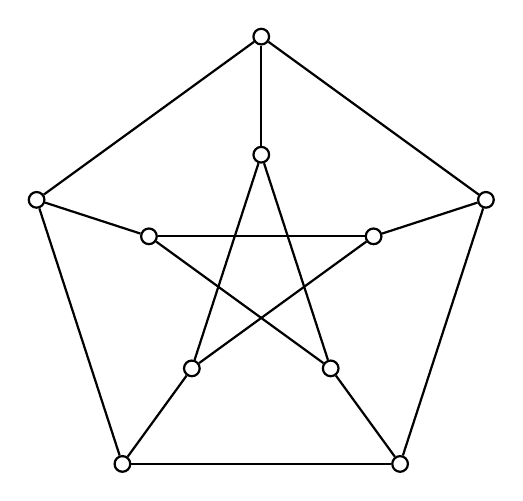
\begin{tikzpicture}
[nodeDecorate/.style={shape=circle,inner sep=2pt,draw,thick},%
  lineDecorate/.style={-,thick},scale=1.5]
%% nodes or vertices
\foreach \nodename/\x/\y in {
  %% outer pentagon
  0/0/2, 1/-1.9021/0.6180, 2/-1.1755/-1.6180, 3/1.1755/-1.6180,
  4/1.9021/0.6180,
  %% inner pentagon
  5/0/1, 6/-0.9510/0.3090, 7/-0.5877/-0.8090, 8/0.5877/-0.8090,
  9/0.9510/0.3090}
{
  \node (\nodename) at (\x,\y) [nodeDecorate] {};
}
%% edges or lines
\path
\foreach \startnode/\endnode in {0/1, 0/4, 0/5, 1/2, 1/6, 2/3, 2/7,
  3/4, 3/8, 4/9, 5/7, 5/8, 6/8, 6/9, 7/9}
{
  (\startnode) edge[lineDecorate] node {} (\endnode)
};
\end{tikzpicture}
\end{figure}

\end{document}

\caption{The Petersen graph with $10$ vertices.}
\label{fig:distance_connectivity:petersen_graph}
\end{figure}
}
\end{example}
The the minimum degree of a graph $G=(V,E)$ is
denoted

\[
\delta(G) = \min_{v\in V} \deg(v).
\]
\index{$\delta(G)$}

\begin{proposition}
{\rm
In general,

\[
\kappa(G)\leq \lambda(G)\leq \delta(G).
\]
}
\end{proposition}

This is called {\it Whitney's inequality}.
\index{Whitney's inequality}

\begin{proof}[Solution]

...

\end{proof}

\begin{theorem}
{\rm
If $G=(V,E)$ is a connected graph with $n=|V|$ and if
$\deg(v)\geq (n+k-2)/2$, for all $v\in V$, then
$G$ is $k$-vertex-connected.
}
\end{theorem}

\begin{proof}[Solution]

...

\end{proof}


\begin{corollary} (Harary)
{\rm
A graph $G=(V,E)$ having $|V|\geq 3$ is a block if and only if
every pair of vertices lie on a common
cycle.
}
\end{corollary}


Recall that a {\it cut-set} or {\it bond}
or {\it cocycle} is a disconnecting set $F$ of a graph $G$ such that
no proper subset of $F$ is also a disconnecting set.
A {\it cut} of $G=(V,E)$ is a subset $C\subset E$ of the form

\[
C=\{e\in E\ \ | e=(x,y), \ x\in S,\ y\in T\}.
\]
where $V=S\cup T$ is a fixed partition.
This cut set is denoted $cut(S,T)$.
\index{$cut(S,T)$}

\begin{lemma}
{\rm
Every cut set is a cut.
}
\end{lemma}

\begin{proof}[Solution]
Let $H$ be a connected subgraph of $G$ obtained after removing from
$G$ all the edges in a cut set $F$. Let $W$ be the set of vertices
of $H$. Then $F=cut(V,V-W)$.
\end{proof}

The converse of this lemma is false.

\begin{theorem}
{\rm
A graph is $k$-edge-connected if and only if the number of
edges in any cut is $\geq k$.
}
\end{theorem}

\begin{proof}[Solution]

...

\end{proof}


Let $G=(V,E)$ be a connected graph and $u,v\in V$ be distinct non-adjacent
vertices. A path from $u$ to $v$ is called a
{\it $u$-$v$ path}.
\index{path!$u$-$v$}
Two paths $P_1$, $P_2$ from $u$ to $v$ are called {\it independent}
(or {\it vertex-disjoint} or {\it internally disjoint} or
{\it vertex-independent}) if there are no vertices
in common between $P_1$ and $P_2$ except $u$ and $v$.
\index{internally disjoint paths}
\index{vertex-disjoint paths}
\index{independent paths}
\index{vertex-independent paths}
Two paths $P_1$, $P_2$ from $u$ to $v$ are called
{\it edge-independent}
{\it edge-disjoint}
if there are no edges
in common between $P_1$ and $P_2$.
\index{edge-disjoint paths}
\index{edge-independent paths}


Let $W$ be a set of vertices or a set of edges.
If $W\subset V$ then we define $G-W$ to be the subgraph
of $G$ which has all the vertices in $W$ and all incident
edges in $E$ removed.  If $W\subset E$ then we define $G-W$ to be the subgraph
of $G$ which has all the edges in $W$ removed
(but not the incident vertices).
If $G-W$ is not connected then we call $W$ a
{\it separating set} and we say $W$ {\it separates} $G$.
\index{separating set}
\index{separates}

\section{Ford-Fulkerson Theorem}

The Ford-Fulkerson Theorem, or ``Max-flow/Min-cut Theorem,''
was proven by P. Elias, A. Feinstein, and C.E. Shannon in 1956, and,
independently, by L.R. Ford, Jr.  and D.R. Fulkerson in the same year.
So it should be called the
``Elias-Feinstein-Ford-Fulkerson-Shannon Theorem,''
to be precise about the authorship.

To explain the meaning of this theorem, we need to introduce some
notation and  terminology.

Consider an edge-weighted simple
digraph $G=(V,E,i,h)$ without negative weight
cycles. Here $E\subset V^{(2)}$,
$i$ is an incidence function as in~\eqref{eqn:edge-incidence}, which
we regard as the identity function, and $h$ is an
orientation function as in~\eqref{eqn:edge-orientation}.
Let $G$ be a {\it network},
\index{network}
with two distinguished vertices, the ``source'' and the ``sink.''
Let $s$ and $t$ denote the source and the sink of $G$, respectively.
The {\it capacity} (or {\it edge capacity})
\index{capacity}
\index{edge capacity})
is a mapping $c: E \to {\mathbf{R}}$, denoted by $c_{uv}$
or $c(u,v)$, for $(u,v)\in E$ and $h(e)= u$.
If $(u,v)\in E$ and $h(e)= v$
then we set, by convention, $c(v,u)=-c(u,v)$.
Thinking of a graph as a network of pipes (representing the edges)
transporting water with various junctions (representing vertices),
the capacity function represents the maximum amount
of ``flow'' that can pass through an edge.

A {\it flow}
\index{flow}
is a mapping $f: E \to {\mathbf{R}}$, denoted by $f_{uv}$ or
$f(u,v)$, subject to the following two constraints:
\begin{itemize}
\item
$f(u,v)\leq c(u,v)$, for each $(u,v) \in V$ (the ``capacity constraint''),
\item
$\sum_{u\in V,\ (u,v)\in E} f(u,v) = \sum_{u\in V,\ (v, u)\in E} f(v, u)$ ,
for each $v\in V$ (conservation of flows).
\end{itemize}
An edge $(u,v) \in E$ is {\it $f$-saturated}
\index{$f$-saturated}
\index{saturated edge}
if $f(u,v)=c(u,v)$.
An edge $(u,v) \in E$ is {\it $f$-zero} if $f(u,v)=0$.
\index{$f$-zero}
A path with available capacity is called an ``augmenting path.''
More precisely, a directed path form $s$ to $t$ is
{\it $f$-augmenting}, or
\index{$f$-augmenting}
\index{$f$-unsaturated}
\index{augmenting path}
$f$-unsaturated, if no forward
edge is $f$-saturated and no backward edge is $f$-zero.

The {\it value of the flow} is defined by

\[
| f | = \sum_{v\in V}f(s,v)-\sum_{v\in V}f(v,s),
\]
where $s$ is the source.
It represents the amount of flow passing from the source to the sink.
\index{flow!value}
\index{value of flow}
The {\it maximum flow problem} is to maximize $| f |$, that is, to route as
much flow as possible from $s$ to $t$.
\index{maximum flow problem}

\begin{example}
{\rm
Consider the digraph having adjacency matrix

\[
\left(\begin{array}{cccccc}
0 & 1 & 1 & 0 & 0 & 0 \\
-1 & 0 & -1 & 1 & 0 & 1 \\
-1 & 1 & 0 & 0 & 1 & 0 \\
0 & -1 & 0 & 0 & 0 & 1 \\
0 & 0 & -1 & 0 & 0 & 1 \\
0 & -1 & 0 & -1 & -1 & 0
\end{array}\right),
\]
depicted in Figure \ref{fig:digraph-flow1}.

\begin{figure}[!htbp]
\centering
\input{image/distance-connectivity/digraph-flow1.tex}
\caption{A digraph with $6$ vertices.}
\label{fig:digraph-flow1}
\end{figure}
Suppose that each edge has capacity $1$.
A maximum flow $f$ is obtained by taking a flow value
of $1$ along each edge of the path

\[
p_1:(0,1),(1,5),
\]
and a flow value
of $1$ along each edge of the path

\[
p_2:(0,2),(2,4),(4,5).
\]
The maximum value of the flow in this case is $|f|=2$.

This graph can be created in Sage using the commands

\begin{lstlisting}
sage: B = matrix([[0,1,1,0,0,0],[0,0,0,1,0,1],[0,1,0,0,1,0],[0,0,0,0,0,1],[0,0,0,0,0,1],[0,0,0,0,0,0]])
sage: H = DiGraph(B, format = "adjacency_matrix", weighted=True)
\end{lstlisting}

\noindent
Type {\tt H.show(edge\_labels=True)} if you want to see the graph with
the capacities labeling the edges.


}
\end{example}


Given a capacitated digraph with capacity $c$ and flow $f$,
we define the {\it residual digraph} $G_f=(V,E)$ to be the
digraph with capacity $c_f(u,v) = c(u,v) - f(u,v)$ and no flow.
In other words, $G_f$ is the same graph but it has a different
capacity $c_f$ and flow $0$.
\index{residual digraph}
This is also called a {\it residual network}.
\index{residual network}

Define an {\it $s-t$ cut} in our capacitated digraph $G$
to be a partition $C = (S,T)$ of $V$ such that
$s \in S$ and $t\in T$.
Recall the cut-set of $C$ is the set

\[
\{(u,v)\in E\ |\ u\in S, v\in T\}.
\]

\begin{lemma}
\label{lemma:flow=0}
{\rm
Let $G = (V, E)$ be a capacitated digraph with
capacity $c: E \to {\mathbf{R}}$, and let
$s$ and $t$ denote the source and the sink of $G$, respectively.
If $C$ is an $s-t$ cut and if
the edges in the cut-set of $C$ are removed, then $| f | = 0$.
}
\end{lemma}

\begin{exercise}
Prove Lemma \ref{lemma:flow=0}.
\end{exercise}

The {\it capacity of an $s-t$ cut}
\index{capacity!cut}
$C = (S,T)$ is defined by

\[
c(S,T) = \sum_{(s,t)\in (S,T)} c(u,v).
\]
The {\it minimum cut problem}
\index{minimum cut problem}
is to minimize the amount of capacity of an $s-t$ cut.

The following theorem is due to P. Elias, A. Feinstein, L.R. Ford,
Jr.,  D.R. Fulkerson, C.E. Shannon.

\begin{theorem}
(max-flow min-cut theorem)
{\rm
The maximum value of an $s$-$t$ flow is equal to the minimum capacity of
an $s$-$t$ cut.
}
\end{theorem}
\index{max-flow min-cut theorem}

The intuitive explanation of this result is as follows.

Suppose that $G=(V,E)$ is a graph where each edge has capacity $1$.
Let $s\in V$ be the source and $t\in V$ be the sink.
The maximum flow from $s$ to $t$ is the maximum number of
independent paths from $s$ to $t$.
Denote this maximum flow by $m$.
Each $s$-$t$ cut must intersect each $s$-$t$ path at least once.
In fact, if $S$ is a minimal $s$-$t$ cut then for each
edge $e$ in $S$ there is an $s$-$t$ path containing
$e$. Therefore, $|S|\leq e$.

On the other hand, since each edge has unit capacity,
the maximum flow value can't exceed the number of
edges separating $s$ from $t$, so $m\leq |S|$.


\begin{remark}
Although the notion of an independent path is important
for the network-theoretic proof of Menger's theorem
(which we view as a corollary to the Ford-Fulkerson
theorem on network flows on networks having
capacity $1$ on all edges), its significance is less
important for networks having arbitrary capacities.
One must use caution in generalizing the above
intuitive argument to establish a rigorous proof
of the general version of the MFMC theorem.
\end{remark}

\begin{remark}
\label{remark:GMCMF}
{\rm
This theorem can be generalized as follows.
In addition to edge capacity, suppose there is capacity at each {\it vertex},
that is, a mapping $c: V \to {\mathbf{R}}$, denoted by
$v \mapsto c(v)$, such that the flow $f$ has to
satisfy not only the capacity constraint and the conservation of flows,
but also the vertex capacity constraint

\[
 \sum_{w\in V} f(w,v) \leq c(v),
\]
for each $v \in V-\{s,t\}$.
Define an {\it $s-t$ cut} to be the set of vertices and edges such
that for any path from $s$ to $t$, the path contains a member of the cut.
In this case, the capacity of the cut is the sum the capacity of each
edge {\it and} vertex in it.
In this new definition, the {\it generalized max-flow min-cut theorem}
\index{max-flow min-cut theorem!generalized}
states that the maximum value of an $s-t$ flow is equal to the minimum
capacity of an $s-t$ cut..
}
\end{remark}

The idea behind the Ford-Fulkerson algorithm is very simple: As long as
there is a path from the source to the sink, with
available capacity on all edges in the
path, we send as much flow as we can alone along each
of these paths. This is done inductively, one path at a time.

\begin{algorithm}[!htbp]
%%%%%%%%%%%%%%%%%%%%%%%%%%%%%%%%%%%%%%%%%%%%%%%%%%%%%%%%%%%%%%%%%%%%%%%%%%%
%% This file is part of the book
%%
%% Algorithmic Graph Theory
%% http://code.google.com/p/graph-theory-algorithms-book/
%%
%% Copyright (C) 2009, 2010 Minh Van Nguyen <nguyenminh2@gmail.com>
%%
%% See the file COPYING for copying conditions.
%%%%%%%%%%%%%%%%%%%%%%%%%%%%%%%%%%%%%%%%%%%%%%%%%%%%%%%%%%%%%%%%%%%%%%%%%%%

\DontPrintSemicolon
\SetAlgoNoLine
%%
%% data section
\SetKwInOut{Input}{Input}
\SetKwInOut{Output}{Output}
%%
%% input/output
\Input{Graph $G=(V,E)$ with flow capacity $c$, source $s$, and sink $t$.}
\Output{A flow $f$ from $s$ to $t$ which is a maximum for all edges in $E$.}
\BlankLine
%%
%% algorithm body
Initialize $f(u,v)=0$, for all edges $(u,v)\in E$\;

While there is a path $p$ from $s$ to $t$ in $G_f$, such that
$c_f(e) > 0$, for all edges $e\in E$:\;
\quad       Find $c_f(p) = min\{ c_f(u,v)\ |\ (u,v) \in p\}$,\;
\quad       For each edge $(u,v) \in $:\;
\quad   \quad        $f(u,v) = f(u,v) + c_f(p)$\;
\quad   \quad        $f(v,u) = f(v,u) - c_f(p)$\;

\caption{Ford-Fulkerson algorithm.}
\label{alg:distance-connectivity:ford-fulkerson}
\end{algorithm}

To prove the max-flow/min-cut theorem we will use the following lemma.

\begin{lemma}
{\rm
Let $G=(V,E)$ be a directed graph with edge
capacity $c: E \to {\mathbf{Z}}$,
a source $s\in V$, and a sink $t\in V$.
A flow $f: E \to {\mathbf{Z}}$ is a maximum flow if
and only if there is no $f$-augmenting path in the graph.
}
\end{lemma}

In other words, a flow $f$ in a
capacitated network is a maximum flow if and only if
there is no $f$-augmenting path in the network.

\begin{proof}[Solution]
One direction is easy. Suppose that the flow is a maximum.
If there is an $f$-augmenting path then the
current flow can be increased using that path, so the flow would not
be a maximum. This contradiction proves the ``only if'' direction.

Now, suppose there is no $f$-augmenting path in the network.
Let $S$ be the set of vertices $v$ such that there is an $f$-unsaturated path from
the source $s$ to $v$. We know $s\in S$ and (by hypothesis)
$t\notin S$. Thus there is a cut of the form $(S,T)$ in the network.
Let $e=(v,w)$ be any edge in this cut, $v\in S$ and $w\in T$. Since
there is no $f$-unsaturated path from $s$ to $w$,
$e$ is $f$-saturated. Likewise, any edge in the cut
$(T,S)$ is $f$-zero. Therefore, the current flow value is equal to the
capacity of the cut $(S,T)$. Therefore, the current flow is a maximum.
\end{proof}

We can now prove the max-flow/min-cut theorem.

\begin{proof}[Solution]
Let $f$ be a maximum flow.
If

\[
S = \{v\in V\ |\ {\rm there\ exists\ an\ }f-{\rm saturated\ path\
  from\ }s\ {\rm to\ }v\},
\]
then by the previous lemma, $S\not= V$.
Since $T=V-S$ is non-empty, there is a cut $C=(S,T)$.
Each edge of this cut $C$ in the capacitated network $G$ is
$f$-saturated.

\end{proof}

Here is some Python code\footnote{Please see
\url{http://en.wikipedia.org/wiki/Ford-Fulkerson_algorithm}.}
which implements this. The class {\tt FlowNetwork} is basically a Sage
Graph class with edge weights and an extra data structure representing
the flow on the graph.

%%%%%%%%%%%%%%%%%%%%%%%%%%%%%%%%%%%%%%%%%%%%%%%%%%
% TODO: Translate this into Sage
%% easiler said than done, since the flow "record" is missing from
%% Sage. One way: create new functions "find_path" and "max_flow"
%% similar to the ones below but with a new argument
%% "flow" which is a function on the edges of G. Maybe there
%% is a better way??
%%%%%%%%%%%%%%%%%%%%%%%%%%%%%%%%%%%%%%%%%%%%%%%%%%
\begin{lstlisting}
class Edge:
    def __init__(self,U,V,w):
        self.source = U
        self.to = V
        self.capacity = w
    def __repr__(self):
        return str(self.source) + "->" + str(self.to) + " : " + str(self.capacity)

class FlowNetwork(object):
    """
    This is a graph structure with edge capacities.

    EXAMPLES:
        g=FlowNetwork()
        map(g.add_vertex, ['s','o','p','q','r','t'])
        g.add_edge('s','o',3)
        g.add_edge('s','p',3)
        g.add_edge('o','p',2)
        g.add_edge('o','q',3)
        g.add_edge('p','r',2)
        g.add_edge('r','t',3)
        g.add_edge('q','r',4)
        g.add_edge('q','t',2)
        print g.max_flow('s','t')
    """
    def __init__(self):
        self.adj, self.flow, = {},{}

    def add_vertex(self, vertex):
        self.adj[vertex] = []

    def get_edges(self, v):
        return self.adj[v]

    def add_edge(self, u,v,w=0):
        assert(u != v)
        edge = Edge(u,v,w)
        redge = Edge(v,u,0)
        edge.redge = redge
        redge.redge = edge
        self.adj[u].append(edge)
        self.adj[v].append(redge)
        self.flow[edge] = self.flow[redge] = 0

    def find_path(self, source, sink, path):
        if source == sink:
            return path
        for edge in self.get_edges(source):
            residual = edge.capacity - self.flow[edge]
            if residual > 0 and not (edge,residual) in path:
                result = self.find_path(edge.to, sink, path + [ (edge,residual) ])
                if result != None:
                    return result

    def max_flow(self, source, sink):
        path = self.find_path(source, sink, [])
        while path != None:
            flow = min(res for edge,res in path)
            for edge,res in path:
                self.flow[edge] += flow
                self.flow[edge.redge] -= flow
            path = self.find_path(source, sink, [])
        return sum(self.flow[edge] for edge in self.get_edges(source))
\end{lstlisting}


%%%%%%%%%%%%%%%%%%%%%%%%%%%%%%%%%%%%%%%%%%%%%%%%%%%%%%%%%%%%%%%%%%%%%%%%%%%

\section{Menger's Theorem}
\index{Menger's theorem}

Menger's theorem has a number of different versions
(a undirected, vertex-connectivity version,
a directed, vertex-connectivity version,
undirected, edge-connectivity version, and
a directed, edge-connectivity version). The following statement
is the undirected, vertex-connectivity version.

\begin{theorem}
\textbf{Menger's Theorem.}
Let $u$ and $v$ be distinct, non-adjacent vertices in an undirected
connected graph
$G$. Then the maximum number of internally disjoint $u$-$v$ paths in
$G$ equals the minimum number of vertices needed to separate $u$ and $v$.
\end{theorem}

\begin{proof}[Solution]
Suppose that the maximum number of independent $u$-$v$ paths in
$G$ is attained by $u$-$v$ paths $P_1$, \dots, $P_k$.
To obtain a separating set $W\subset V$, we must at least remove
one point in each path $P_i$. This implies
the minimum number of vertices needed to separate $u$ and $v$
is at least $k$. Therefore, we have an upper bound:

\[
\#\{ {\rm indep.}\ u-v\ {\rm paths}\}
\leq
\# \{{\rm min.\ number \ of\ vertices\ needed\ to\ separate}\ u\
{\rm and}\  v\}.
\]

We show that equality holds. Let $n$ denote the number
of edges of $G$. The proof is by induction on $n$. By hypothesis,
$n\geq 2$.
If $n=2$ the statement holds by inspection, since in that case
$G$ is a line graph with $3$ vertices
$V=\{u,v,w\}$ and $2$ edges, $E=\{uw.wv\}$. In that situation,
there is only $1$ $u$-$v$ path
(namely, $uwv$) and only one vertex separating $u$ and $v$
(namely, $w$).

Suppose now $n>3$ and assume the statement holds for each
graph with $<n$ edges. Let

\[
k = \#\{ {\rm independent}\ u-v\ {\rm paths}\}
\]
and let
\[
\ell =
\# \{{\rm min.\ number \ of\ vertices\ needed\ to\ separate}\
u\ {\rm and}\  v\},
\]
so that $k\leq \ell$. Let $e\in E$ and let $G/e$ be the
contraction graph having edges $E-\{e\}$ and
vertices the same as those of $G$, except that
the endpoints of $e$ have been identified.

Suppose that $k<\ell$ and $G$ does not have $\ell$
independent $u$-$v$ paths. The contraction
graph $G/e$ does not have $\ell$
independent $u$-$v$ paths either (where
now, if $e$ contains $u$ or $v$ then we must
appropriately redefine $u$ or $v$, if needed).
However, by the induction hypothesis
$G/e$ does have the property that
the maximum number of internally disjoint $u$-$v$ paths
equals the minimum number of vertices needed to separate $u$ and $v$.
Therefore,

\[
\begin{array}{c}
\#\{ {\rm independent}\ u-v\ {\rm paths\ in}\ G/e\}\\
<
\# \{{\rm min.\ number \ of\ vertices\ needed\ to\ separate}
\ u\ {\rm and}\  v\ {\rm in}\ G\}.
\end{array}
\]
By induction,

\[
\begin{array}{c}
\#\{ {\rm independent\ }u-v{\rm \ paths\ in\ }G/e\}\\
=
\# \{{\rm min.\ number \ of\ vertices\ needed\ to\ separate\
}u{\rm \ and}\  v\ {\rm in\ }G/e\}.
\end{array}
\]

Now, we {\it claim} we can pick $e$ such that $e$ does contain $u$ or $v$
and in such a way that

\[
\begin{array}{c}
\# \{{\rm minimum\ number \ of\ vertices\ needed\ to\ separate\ }u\
{\rm and\  }v\ {\rm in\ }G\}\\
\geq
\# \{{\rm minimum\ number \ of\ vertices\ needed\ to\ separate\ }u\
{\rm and\  }v\ {\rm in}\ G/e\}.
\end{array}
\]
Proof: Indeed, since $n>3$ any separating set realizing
the minimum number  of vertices needed to separate $u$ and
$v$ in $G$ cannot contain both a vertex in $G$ adjacent to $u$ and a vertex in
$G$ adjacent to $v$. Therefore, we may pick $e$ accordingly.
(Q.E.D. claim)

The result follows from the claim and the above inequalities.
\end{proof}

The following statement
is the undirected, edge-connectivity version of
Menger's theorem.

\begin{theorem}
\textbf{Menger's theorem (edge-connectivity form).}
{\rm
Let $G$ be an undirected graph, and let $s$ and $t$ be vertices in
$G$.
Then, the maximum number of edge-disjoint $(s,t)$-paths in
$G$
equals the minimum number of edges from $E(G)$ whose
deletion separates $s$ and $t$.
}
\end{theorem}

This is proven the same way as the previous version
but using the generalized min-cut/max-flow theorem (see
Remark \ref{remark:GMCMF} above).


%%%%%%%%%%%%%%%%%%%%%%%%%%%%%%%%%%%%%%%%%%%%%%%%%%%%%%%%%%%%%%%%%%%%%%%%%%%

\section{Whitney's Theorem}
\index{Whitney's Theorem}

\begin{theorem}
\textbf{Whitney's theorem (vertex version).}
{\rm
Suppose $G=(V,E)$ is a graph with $|V|\geq k+1$. The following are
equivalent:
\begin{itemize}
\item
$G$ is $k$-vertex-connected,
\item
Any pair of distinct vertices $v,w\in V$ are connected by
at least $k$ independent paths.
\end{itemize}
}
\end{theorem}

\begin{proof}[Solution]

...

\end{proof}



\begin{theorem}
\textbf{Whitney's theorem (edge version).}
{\rm
Suppose $G=(V,E)$ is a graph with $|V|\geq k+1$. The following are
equivalent:
\begin{itemize}
\item
the graph $G$ is $k$-edge-connected,

\item
any pair of
vertices are connected by at least $k$ edge-disjoint paths.
\end{itemize}
}
\end{theorem}

\begin{proof}[Solution]

...

\end{proof}


\begin{theorem}
\textbf{Whitney's Theorem.}
Let $G = (V, E)$ be a connected graph such that $|V| \geq 3$. Then $G$
is $2$-connected if and only if any pair $u,v \in V$ has two
internally disjoint paths between them.
\end{theorem}


%%%%%%%%%%%%%%%%%%%%%%%%%%%%%%%%%%%%%%%%%%%%%%%%%%%%%%%%%%%%%%%%%%%%%%%%%%%

\section{Centrality of a vertex}

\begin{itemize}
\item degree centrality

\item betweenness centrality

\item closeness centrality

\item eigenvector centrality
\end{itemize}

\begin{algorithm}[!htbp]
\index{friendship graph}
%%%%%%%%%%%%%%%%%%%%%%%%%%%%%%%%%%%%%%%%%%%%%%%%%%%%%%%%%%%%%%%%%%%%%%%%%%%
%% This file is part of the book
%%
%% Algorithmic Graph Theory
%% http://code.google.com/p/graph-theory-algorithms-book/
%%
%% Copyright (C) 2009, 2010 Minh Van Nguyen <nguyenminh2@gmail.com>
%%
%% See the file COPYING for copying conditions.
%%%%%%%%%%%%%%%%%%%%%%%%%%%%%%%%%%%%%%%%%%%%%%%%%%%%%%%%%%%%%%%%%%%%%%%%%%%

\DontPrintSemicolon
\SetAlgoNoLine
%%
%% data section
\SetKwInOut{Input}{Input}
\SetKwInOut{Output}{Output}
%%
%% input/output
\Input{A positive integer $n$.}
\Output{An edge list $E$ containing the edges of the friendship graph
  $F_n$.}
\BlankLine
%%
%% algorithm body
\If{$n = 1$}{
  \Return $C_3$\;
}
$E \assign [\,]$\;
$N \assign 2n + 1$\;
\For{$i \assign 0, 1, \dots, N-3$}{
  \eIf{\rm $i$ is odd}{
    append to $E$ the edges $(i,\, i+1)$ and $(i,\, N-1)$\;
  }{
    append to $E$ the edge $(i, N-1)$\;
  }
}
append to $E$ the edges $(N-2,\, 0)$ and $(N-2,\, N-1)$\;
\Return $E$\;

\caption{Friendship graph.}
\label{alg:distance_connectivity:friendship_graphs}
\end{algorithm}


%%%%%%%%%%%%%%%%%%%%%%%%%%%%%%%%%%%%%%%%%%%%%%%%%%%%%%%%%%%%%%%%%%%%%%%%%%%

\section{Network reliability}

\begin{itemize}
\item Whitney synthesis

\item Tutte's synthesis of $3$-connected graphs

\item Harary graphs

\item constructing an optimal $k$-connected $n$-vertex graph
\end{itemize}
